\documentclass{beamer}
\usetheme[shownavsym]{AAUsimple}
\usefonttheme{structurebold}
%%%%%%%%%%%%%%%%%%%%%%%%%%%%%%%%%%
\usepackage[utf8]{inputenc}
\usepackage[T1]{fontenc}
\usepackage[dutch]{babel}
\usepackage{tikz}
\usetikzlibrary{positioning,calc,intersections}
\usepackage{hyperref}
\usepackage{microtype}
\usepackage{array,multirow, booktabs}%%Tabellenmaker 1.Array voor horizontale lijn en arraystretch, 2. Multirow en Multicolumn voor merging rijen en columnen respectievelijk, 3.Booktabs voor code commands in tabel.
\renewcommand{\arraystretch}{1.5}%Ruimte tussen twee rijen
\setlength{\tabcolsep}{10pt}%Ruimte tussen twee colommen 
%%%%%%%%%%%
\definecolor{darkblue}{RGB}{33,26,82}
\definecolor{lightblue}{RGB}{194,193,204}
%%%%%%%%%%%%%%%%%%%%%%%%%%%%%%%%%%
% Gekleurde hyperlinks
\newcommand{\chref}[2]{%
	\href{#1}{{\usebeamercolor[bg]{AAUsidebar}#2}}%
}
\title[Tutor1]{Mitose  \& Me\"iose}

\date{\today}

\author[Edon Namani, et. al]
{%
	Edon Namani\\
	\href{mailto:e.namani@student.rug.nl}{{\tt e.namani@student.rug.nl}}
}

\institute[%
	Faculteit Gezondheidswetenschappen\\
	Rijksuniversiteit Groningen\\
	Nederland
]
{%
	Faculteit Gezondheidswetenschappen\\
	Rijksuniversiteit Groningen\\
	Nederland

}

\pgfdeclareimage[height=1.5cm]{titlepagelogo}{AAUgraphics/semper_invicta.pdf}
\titlegraphic{%
	\pgfuseimage{titlepagelogo}
}

\begin{document}
% Titel
{\aauwavesbg%
	\begin{frame}[plain,noframenumbering]
	\titlepage
\end{frame}}
%%%%%%%%%%%%%%%

%TOC
\begin{frame}{Agenda}{}
	\tableofcontents
\end{frame}
%%%%%%%%%%%%%%%

%Mitosis
\section{Mitose}
\begin{frame}{Mitose}
	\begin{block}{Doel mitosis}
		Gelijke verdeling van het in de S-fase verdubbelde DNA over twee cellen. Deze verdeling gebeurt in 5 stappen.
	\end{block}
\end{frame}
%%%

\subsection{Profase}
\begin{frame}{Mitose}{Profase}
	\begin{minipage}{.5\textwidth}
	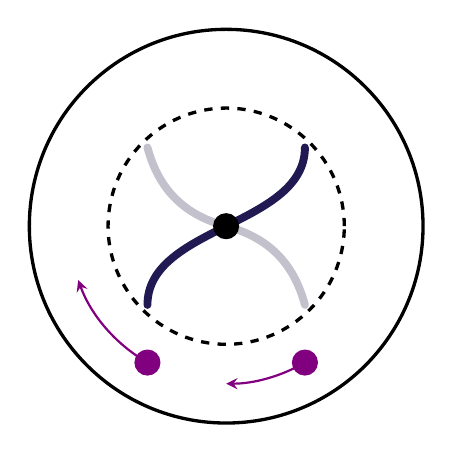
\begin{tikzpicture}[chrom/.style={line width=1mm,cap=round,color=darkblue}]
%		\draw[lightgray] (-3,-3) grid (3,3);
%		\foreach \x in {0,1,...,3}
%		\draw (\x,1mm) -- (\x,-1mm);
%		\foreach \y in {0,1,...,3}
%		\draw (1mm,\y) -- (-1mm,\y);
		\draw[very thick] circle (2.5cm);
		\draw[very thick,dashed] circle (1.5cm);
		\draw[name path=chrom1,chrom] (-1,-1) .. controls (-1,0) and (1,0) .. (1,1);
		%\draw[name path=chrom2,chrom,color=lightblue] (-1,0) .. controls (-.5,1) .. (0,0) .. controls (0,-1) .. (1,-1);
		\draw[name path=chrom2,chrom,color=lightblue] (-1,1) to[bend right] (0,0) to[bend left] (1,-1);
		\path[name intersections={of=chrom1 and chrom2, by=intersec}];
		\node[circle,fill] at (intersec) {};
		\node[circle,fill,violet] at (-120:2) {};
		\node[circle,fill,violet] at (-60:2) {};
		\draw[thick,->,>=stealth,violet] (-120:2)  arc[start angle=-120, end angle=-160,radius=2cm];
		\draw[thick,->,>=stealth,violet] (-60:2)  arc[start angle=-60, end angle=-90,radius=2cm];
	\end{tikzpicture}
\end{minipage}
\hfill
\begin{minipage}{.45\textwidth}
	\begin{block}{kenmerken}
		\begin{itemize}
		\item Kernmembraan verdwijnt
		\item Centrosomen verdubbelen en bewegen naar de polen
		\end{itemize}
	\end{block}
\end{minipage}
\end{frame}

\subsection{Metafase}
\begin{frame}{Mitose}{Profase}
	\begin{minipage}{.5\textwidth}
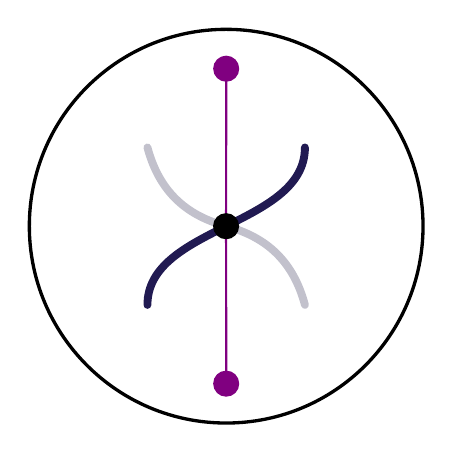
\begin{tikzpicture}[chrom/.style={line width=1mm,cap=round,color=darkblue}]
%		\draw[lightgray] (-3,-3) grid (3,3);
%		\foreach \x in {0,1,...,3}
%		\draw (\x,1mm) -- (\x,-1mm);
%		\foreach \y in {0,1,...,3}
%		\draw (1mm,\y) -- (-1mm,\y);
		\draw[very thick] circle (2.5cm);
		\draw[name path=chrom1,chrom] (-1,-1) .. controls (-1,0) and (1,0) .. (1,1);
		%\draw[name path=chrom2,chrom,color=lightblue] (-1,0) .. controls (-.5,1) .. (0,0) .. controls (0,-1) .. (1,-1);
		\draw[name path=chrom2,chrom,color=lightblue] (-1,1) to[bend right] (0,0) to[bend left] (1,-1);
		\path[name intersections={of=chrom1 and chrom2, by=intersec}];
		\draw[thick,violet] (90:2) -- (intersec);
		\draw[thick,violet] (-90:2) -- (intersec);
		\node[circle,fill] at (intersec) {};
		\node[circle,fill,violet] at (90:2) {};
		\node[circle,fill,violet] at (-90:2) {};
	\end{tikzpicture}
	\end{minipage}
	\hfill
	\begin{minipage}{.45\textwidth}
		\begin{block}{kenmerken}
			\begin{itemize}
				\item Chromosomen op zijn dikst
				\item Chromosomen op equitoriaal vlak gebracht door "spindle apparaat"
			\end{itemize}
		\end{block}
	\end{minipage}
\end{frame}
%%%
\subsection{Anafase}
\begin{frame}{Mitose}{Anafase}
	\begin{minipage}{.5\textwidth}
\begin{tikzpicture}[chrom/.style={line width=1mm,cap=round,color=darkblue}]
%		\draw[lightgray] (-3,-3) grid (3,3);
%		\foreach \x in {0,1,...,3}
%		\draw (\x,1mm) -- (\x,-1mm);
%		\foreach \y in {0,1,...,3}
%		\draw (1mm,\y) -- (-1mm,\y);
		\draw[very thick] circle (2.5cm);
		\draw[name path=chrom1,chrom] (-.9,0) to[bend left] (0,1) to[bend left] (.9,0);
		%\draw[name path=chrom2,chrom,color=lightblue] (-1,0) .. controls (-.5,1) .. (0,0) .. controls (0,-1) .. (1,-1);
		\draw[name path=chrom2,chrom,color=lightblue] (-1,0) to[bend right] (0,-1) to[bend right] (1,0);
		\path[name intersections={of=chrom1 and chrom2, by=intersec}];
		\draw[thick,violet] (90:2) -- (0,1);
		\draw[thick,violet] (-90:2) -- (0,-1);
		%\node[circle,fill] at (intersec) {};
		\node[circle,fill] at (0,-1) {};
		\node[circle,fill] at (0,1) {};
		\node[circle,fill,violet] at (90:2) {};
		\node[circle,fill,violet] at (-90:2) {};
	\end{tikzpicture}
	\end{minipage}
	\hfill
	\begin{minipage}{.45\textwidth}
		\begin{block}{kenmerken}
			\begin{itemize}
				\item De zusterchromatiden worden losgekoppeld. Elke chromatide is nu een chromosoom.
				\item Deze chromosomen worden naar de overstaande polen overgebracht.
			\end{itemize}
		\end{block}
	\end{minipage}
\end{frame}
\subsection{Telofase \& Cytokinese}
\begin{frame}{Mitose}{Telofase \& Cytokinese}
	\begin{minipage}{.5\textwidth}
\begin{tikzpicture}[chrom/.style={line width=1mm,cap=round,color=darkblue}]
%		\draw[lightgray] (-3,-3) grid (3,3);
%		\foreach \x in {0,1,...,3}
%		\draw (\x,1mm) -- (\x,-1mm);
%		\foreach \y in {0,1,...,3}
%		\draw (1mm,\y) -- (-1mm,\y);
		\draw[very thick] circle (2.5cm);
		\draw[name path=chrom1,chrom] (-.9,1) to[bend left] (0,2) to[bend left] (.9,1);
		%\draw[name path=chrom2,chrom,color=lightblue] (-1,0) .. controls (-.5,1) .. (0,0) .. controls (0,-1) .. (1,-1);
		\draw[name path=chrom2,chrom,color=lightblue] (-1,-1) to[bend right] (0,-2) to[bend right] (1,-1);
		\path[name intersections={of=chrom1 and chrom2, by=intersec}];
		%\node[circle,fill] at (intersec) {};
		\node[circle,fill] at (0,-2) {};
		\node[circle,fill] at (0,2) {};
		\node[circle,fill,violet] at (190:2) {};
		\node[circle,fill,violet] at (-190:2) {};
		\draw[very thick] (0,-1.25) circle (1.2cm);
		\draw[very thick] (0,1.25) circle (1.2cm);
		\draw[dashed] (-2.5,0) -- ++ (5,0);
	\end{tikzpicture}
	\end{minipage}
	\hfill
	\begin{minipage}{.45\textwidth}
		\begin{block}{kenmerken}
			\begin{itemize}
				\item Chromosomen worden weer losgewikkeld.
				\item Hervorming van kernmembraan.
				\item Afbraak van "spindle apparaat"
				\item Splitsing van het cytoplasma.
			\end{itemize}
		\end{block}
	\end{minipage}
\end{frame}

\section{Me\"iose}
\begin{frame}{Me\"iose}
	\begin{minipage}{.5\textwidth}
	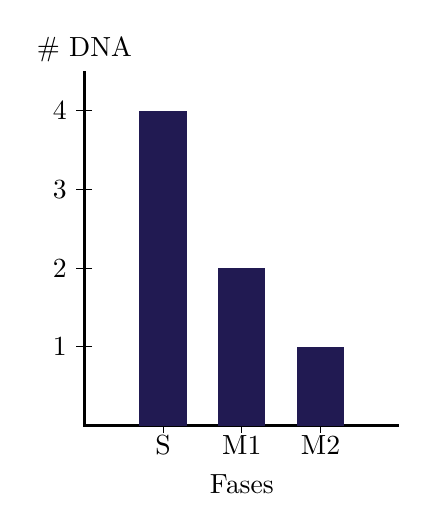
\begin{tikzpicture}
		\foreach \y in {1,2,...,4}
		\draw (1mm,\y) -- (-1mm,\y) node[anchor=east] {\y};
		\foreach \x in {1,2,...,3}
		\draw (\x,1mm) -- (\x,-1mm);
		\draw[very thick] (0,4.5) -- ++(0,-4.5) -- ++(4,0);
		\node[anchor=north] at (1,0) {S};
		\node[anchor=north] at (2,0) {M1};
		\node[anchor=north] at (3,0) {M2};
		\fill[color=darkblue] (.7,0) rectangle (1.3,4);
		\fill[color=darkblue] (1.7,0) rectangle (2.3,2);
		\fill[color=darkblue] (2.7,0) rectangle (3.3,1);
		\node[anchor=south] at (0,4.5) {\# DNA};
		\node[anchor=north] at (2,-.5) {Fases};
	\end{tikzpicture}
\end{minipage}
\hfill
\begin{minipage}{.45\textwidth}
	\begin{block}{Doel}
		\begin{itemize}
			\item Vorming van gameten.
			\item Vergelijkbaar met twee achtereenvolgende mitoses
			\item Belangrijke uitzondering is crossing-over principe tussen \textbf{homologe chromosomen}.
		\end{itemize}
	\end{block}
\end{minipage}
\end{frame}
%%% 
\subsection{Cross-over}
\begin{frame}{Me\"iose}{Crossing-over}
	\begin{minipage}{.5\textwidth}
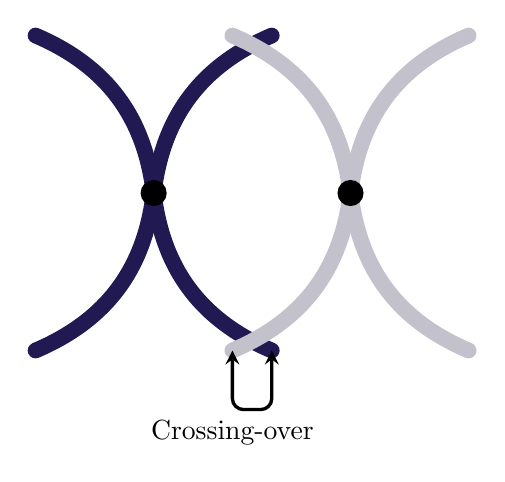
\begin{tikzpicture}[chrom/.style={line width=2mm,cap=round,color=darkblue}]
		%\foreach \y in {1,2,...,5}
		%\draw (1mm,\y) -- (-1mm,\y) node[anchor=east] {\y};
		%\foreach \x in {1,2,...,5}
		%\draw (\x,1mm) -- (\x,-1mm) node[anchor=north] {\x};
	%\draw (0,0) grid (5,5);
	\draw[chrom] (0,1) to[bend right] (1.5,3) to[bend right] (0,5);
	\draw[chrom] (3,1) to[bend left] (1.5,3) to[bend left] (3,5);
	\node[fill,circle] at (1.5,3) {};
	\draw[chrom,color=lightblue] (2.5,1) to[bend right] (4,3) to[bend right] (2.5,5);
	\draw[chrom,color=lightblue] (5.5,1) to[bend left] (4,3) to[bend left] (5.5,5);
	\node[fill,circle] at (4,3) {};
	\draw[very thick,>=stealth,<->,rounded corners] (2.5,1) -- ++(0,-.75) node[anchor=north] {Crossing-over} -| (3,1);
	\end{tikzpicture}
\end{minipage}
\hfill
\begin{minipage}{.45\textwidth}
	\textbf{Crossing-over tussen homologe chromosomen is recombinatie.}
\end{minipage}
\end{frame}
\section{Caveat}
\begin{frame}{Caveat}
	\only<1>{\begin{tabular}{*5c}
		\toprule
		Celdeling & Profase  & Metafase & Anafase & Telofase\\
		\midrule
		Mitose & 46 & 46 & 92 & 92\\
		Me\"iose I & 46 & 46 & 46 & 46\\
		Me\"iose II & 23 & 23 & 46 & 46\\
		\bottomrule
	\end{tabular}
}
\only<2>{Bij vrouwelijke me\"iose neemt maar \'e\'en prematuur gameet alle voeding tot zich en ontwikkelt zich tot een gameet.}
\end{frame}
{\aauwavesbg
\begin{frame}[plain,noframenumbering]
	\finalpage{Vragen?}
\end{frame}}
\end{document}
